% =====================================================================
\part{Transferts de chaleur}
% =====================================================================

\chapter{Conduction}
\label{chap:conduction}

\section{Mécanisme de la conduction}

\section{Loi de Fourier}
\label{sec:fourier}

% --- Exemple à conserver ou à remplacer : équation numérotée, renvoi, figure ---
En régime permanent, dans une paroi plane homogène d'épaisseur $e$ et de conductivité thermique $\lambda$, la densité de flux traversant la paroi est proportionnelle à l'écart de température entre ses deux faces :
\begin{equation}
  \varphi = \frac{\lambda}{e}\,(\theta_1 - \theta_2) = \frac{\Delta\theta}{R}
  \label{eq:fourier}
\end{equation}
où $R = e/\lambda$ est la résistance thermique de la couche, en $\mathrm{m^2{\cdot}K/W}$.

Dans chaque couche, la température varie linéairement, avec une pente d'autant plus forte que le matériau est isolant (figure~\ref{fig:profil}).

\begin{figure}[htbp]
  \centering
  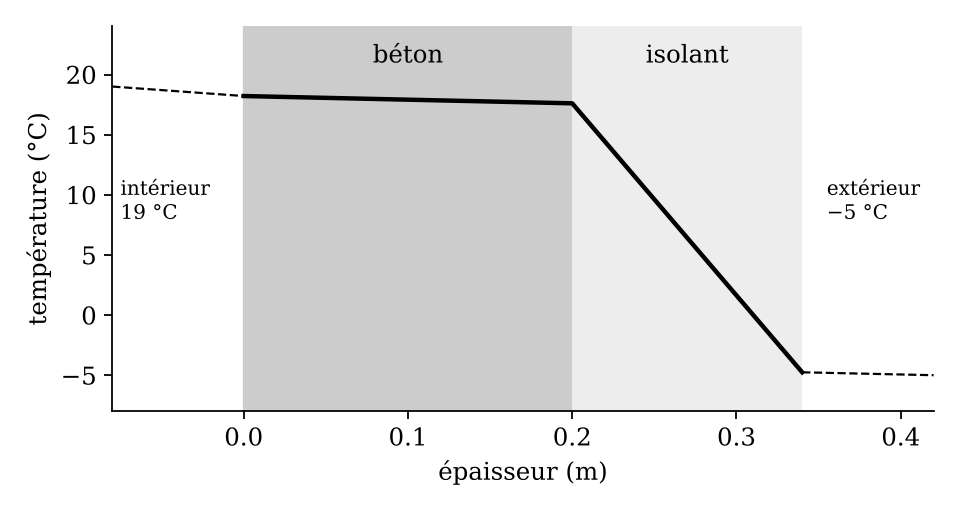
\includegraphics[width=0.7\linewidth]{figures/profil-temperature.png}
  \caption{Profil de température dans un mur en béton isolé par l'extérieur.}
  \label{fig:profil}
\end{figure}
% --- Fin de l'exemple ---

\section{Conduction dans les parois}

\section{Ponts thermiques}

\section{Isolation}

\section{Exercices}

\begin{exercice}
Un mur est composé de 20~cm de béton ($\lambda = 2{,}0\unite{W/(m{\cdot}K)}$) et de 14~cm de laine de bois ($\lambda = 0{,}038\unite{W/(m{\cdot}K)}$). Calculer la résistance thermique de chaque couche à l'aide de l'équation~\eqref{eq:fourier}.
\end{exercice}

\begin{corrige}
Béton : $R = 0{,}20 / 2{,}0 = 0{,}10\unite{m^2{\cdot}K/W}$. Laine de bois : $R = 0{,}14 / 0{,}038 \approx 3{,}68\unite{m^2{\cdot}K/W}$.
\end{corrige}

\chapter{Convection}
\label{chap:convection}

\section{Mécanisme de la convection}

\section{Convection naturelle et convection forcée}

\section{Convection dans le bâtiment}

\chapter{Rayonnement}
\label{chap:rayonnement}

\section{Mécanisme du rayonnement}

\subsection{Le Soleil}

\subsection{Les ondes électromagnétiques}

\section{Apports solaires}

\section{Rayonnement dans le bâtiment}

\chapter{Conclusion sur les transferts de chaleur}
